\documentclass[margin=2cm]{standalone}

\usepackage{tikz,xcolor}
\usetikzlibrary{positioning}

\makeatletter
\tikzset{
  shift to anchor/.code={
    \tikz@scan@one@point\pgfutil@firstofone(-\tikz@anchor)\relax
    \pgfkeysalso{shift={(-\pgf@x,-\pgf@y)}}
  }
}
\makeatother

\begin{document}
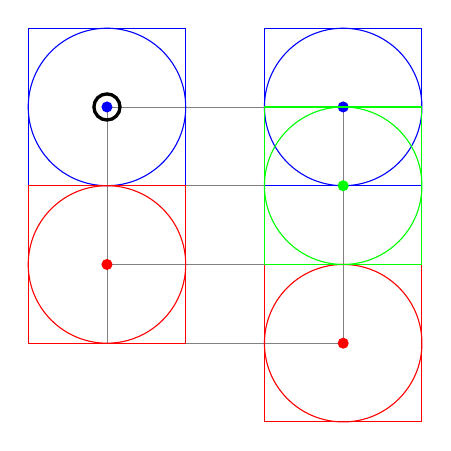
\begin{tikzpicture}[
    pics/test/.style n args={0}{
        code={
            \coordinate (-north) at (0,1);
            \coordinate (-south) at (0,-1);
            \coordinate (-center) at (0,0);
            \begin{scope}[shift to anchor]
                \node[minimum width=2cm, minimum height=2cm,draw,anchor=center]  at (0,0) {};
                \draw[] (0,0) circle (1cm);
                \fill (0,0) circle[radius=2pt];
            \end{scope}
        }       
    }]

    \draw[help lines] (0,0) grid (3,-3);
    \node[circle,draw,very thick] at (0,0) {};

    \pic[blue] (A) at (0, 0) {test};
    \pic[red,below=1cm of A-south,anchor=center] (B) {test};

    \pic[blue] (C) at (3, 0) {test};
    \pic[red,below=1cm of C-south,anchor=north] (D) {test};
    \pic[green,anchor=north] (D) at (3,0) {test};

\end{tikzpicture}
\end{document}